% ============================ 封面区 ============================
\begin{center}
{\LARGE\bfseries\color{accent} 虚拟细胞：面向酿酒酵母扰动蛋白质组的}\\[0.25em]
{\LARGE\bfseries\color{accent} 机制受限预测系统与可质询的探索环境}\\[0.7em]
{\large GOAI 世界人工智能开源大赛 · 赛道三「前沿探索 AI for Research」}\\[0.25em]
{\large 算法赛题一：虚拟细胞 \quad|\quad 初赛方案说明文档}\\[0.25em]
{\normalsize\color{newrule}\bfseries 依据《赛道三 · 虚拟细胞方向参赛规则细化说明》（2026 年 8 月 11 日）修订}\\[0.5em]
\rule{0.86\textwidth}{0.9pt}
\end{center}
\vspace{-0.3em}

\begin{keybox}[title=一句话概括]
\small
我们把「预测细胞对扰动的响应」这一命题，转化为一个\textbf{可计算、可验证、可复现}的探索闭环：先用质控证明数据的三重错配（左删失的测量、批次主导的方差、秩亏的机制），再离线重建官方评测口径并把它变成可以被质询的探索环境，然后把\textbf{化合物结构与作用机制}这两类外部实体表征以\emph{可证伪}的方式注入机制受限的双轨模型，最后由一个不许触碰验证集的自演化环路完成搜索。
验证集总分 \textbf{0.508655}，较按官方分组实现的均值基线 0.445443 高 \textbf{14.2\,\%}；\NEW{}依据修订后释放的测试集真值，我们用同一套离线口径在测试队列上自评得 \textbf{0.463638}，同口径基线 0.424883，\textbf{同一结论在两个独立队列上同向成立}。同时我们如实报告三项\textbf{负结果}、两个未达成的预注册目标，以及一处\textbf{尚未补齐的关键短板}——菌株基因组表征。
\end{keybox}

\vspace{-0.2em}
\begin{figure}[H]
\centering
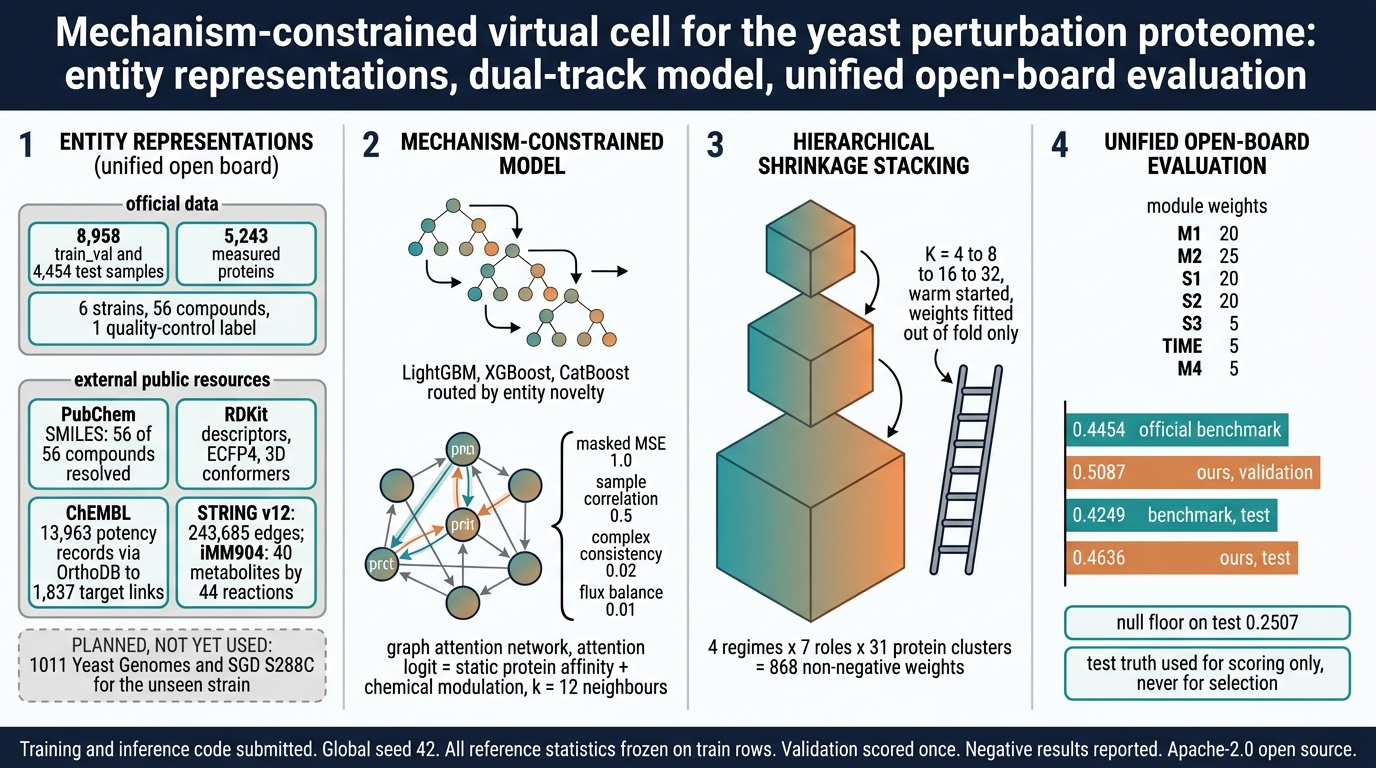
\includegraphics[width=\textwidth]{figures/graphical_abstract_revision.png}
\caption{\textbf{图形摘要：统一开放榜下的机制受限虚拟细胞。} 四个板块依次为——
\textbf{（1）实体表征}：官方四文件（\code{train\_val} 8\,958 例、\code{test} 4\,454 例、5\,243 蛋白；6 菌株、56 化合物与 1 个质控标签）与外部公开资源（PubChem SMILES 56/56 全部解析、RDKit 描述子与三维构象、ChEMBL 13\,963 条效力记录经 OrthoDB 得 1\,837 条靶点连边、STRING v12 的 243\,685 条边、iMM904 的 40 代谢物 $\times$ 44 反应）；灰色虚线框为\emph{已声明但当前尚未使用}的 1011 酵母基因组与 SGD S288C。
\textbf{（2）机制受限模型}：按实体新颖性路由的梯度提升成员，与注意力对数由「静态蛋白亲和 $+$ 化学调制」构成的图注意力成员，损失含四项（掩码 MSE 1.0、逐样本相关 0.5、复合物一致性 0.02、通量平衡 0.01）。
\textbf{（3）分层收缩 stacking}：$4$ 情形 $\times\,7$ 角色 $\times\,31$ 蛋白簇 $=868$ 个非负权重，$K=4\!\to\!8\!\to\!16\!\to\!32$ 逐级热启动，权重\emph{只}在折外队列上拟合。
\textbf{（4）统一开放榜评测}：七模块权重、我方与基线在验证与测试两个队列上的总分，以及测试队列的零假设下限。
底栏为贯穿全程的纪律声明。本图为\emph{概念示意}，其中每一处数字均与正文表格逐项交叉核对；承载定量结论的图件（图 \ref{fig:selfscore}、\ref{fig:entity}、\ref{fig:baselines} 等）一律由脚本从结果产物直接绘制。}
\label{fig:ga}
\end{figure}

% ---------- 修订响应对照 ----------
\begin{table}[H]
\centering
\small
\caption{\textbf{2026-08-11 规则细化说明的四项变化与本文档的响应。} 这张表是本次修订版相对上一版的全部实质差异索引；每一行的「本方案的响应」都指向可核查的产物或章节，而非声明。}
\label{tab:revision}
\begin{tabularx}{\textwidth}{@{}R{2.5cm}R{4.3cm}XR{2.35cm}@{}}
\toprule
\textbf{修订条目} & \textbf{规则变化} & \textbf{本方案的响应（可核查）} & \textbf{落点} \\
\midrule
\textbf{一、两榜合并为统一开放榜} &
外推任务天然需要外部实体表征；不引入则未见实体只能当空白类别处理。 &
我们的化合物侧\emph{本就}走推荐路径：PubChem 检索 SMILES $\to$ RDKit 描述子，56/56 分子标签全部解析；机制侧另有 ChEMBL$\to$OrthoDB 的靶点效力向量。\textbf{菌株侧确为空白类别}——我们据此把「菌株基因组表征」列为下一阶段第一优先，并给出量化判据。 &
\S\ref{sec:entity}；图 \ref{fig:entity}、\ref{fig:itpv}；表 \ref{tab:external} \\
\addlinespace[2pt]
\textbf{二、外部公开数据的来源与版本须披露} &
推荐 PubChem / RDKit、1011 酵母基因组、SGD S288C（DHY210 代理）。 &
外部资源披露清单由脚本\emph{从产物生成}（\file{51\_external\_data\_manifest.py}），含版本、访问时间、许可、计数与「是否影响成绩」；对两项\emph{尚未使用}的基因组资源明确标注「计划使用、当前未用」。 &
表 \ref{tab:external}；\file{evidence/step7\_external\_data\_manifest.json} \\
\addlinespace[2pt]
\textbf{三、初赛须提交训练与推理源代码} &
种子与关键参数在代码中体现；外部资源注明来源与版本；不要求环境打包。 &
随本文档提交 \textbf{73 个科学脚本}与 1 个共享路径模块；主要随机训练阶段固定种子 42，公开 70 份结构化产物摘要与 1 份哈希索引，使评审可在\emph{不重跑}的前提下核对报告结论。 &
\S\ref{sec:repro}；表 \ref{tab:code}、\ref{tab:deps} \\
\addlinespace[2pt]
\textbf{四、新增「开源贡献」维度（占 5\,\%）} &
须说明开源范围、协议、第三方依赖、商业 API、闭源模型、数据来源与授权边界。 &
六项要求逐项作答，并给出\textbf{三个可被他人复核或复用}的组件（评分 harness、快速代理评分器、ITPV 构建与验证流程）；完整 ITPV 未随公开仓库发布，边界单列说明。 &
\S\ref{sec:oss}；表 \ref{tab:oss}、\ref{tab:disclosure} \\
\midrule
\multicolumn{4}{@{}p{\dimexpr\textwidth-2\tabcolsep}@{}}{\emph{另落实的口径细化：}测试集真值随数据包释放（\S\ref{sec:selfscore}，本次\textbf{新增测试队列七模块自评}）；\code{split\_final} 冻结、不改动官方 train/val 边界（\S\ref{sec:protocol}）；\code{test\_time} 为\textbf{时间插值}而非外推（\S\ref{sec:timeinterp}，与我们阶段 2 的独立发现一致）；质控样本 \code{pert\_id = 48} 单列、不计入 56 种化合物（\S\ref{sec:spec}）；提交仅接受 log$_2$ 尺度、蛋白列与 feature contract 完全一致（表 \ref{tab:gates}）。} \\
\bottomrule
\end{tabularx}
\end{table}

% ---------- 评审维度对照 ----------
\begin{table}[H]
\centering
\small
\caption{\textbf{与修订后四个评审维度的对照（权重为修订后口径）。} 每行给出「本方案交付了什么」与「可核查的证据落点」。}
\label{tab:rubricmap}
\begin{tabularx}{\textwidth}{@{}R{3.25cm}XR{3.5cm}@{}}
\toprule
\textbf{评审维度（权重）} & \textbf{本方案的交付} & \textbf{证据落点} \\
\midrule
问题定义与环境设计质量\newline\textbf{（45\,\%）} &
把「虚拟细胞」收敛为有明确失败模式的可计算命题：三重错配（测量/方差/可识别性），每一重给出定量证据；离线重建官方七模块口径（57 项自检、逐位复现基线 0.445443），给出\textbf{两个队列}的零假设下限，并证明 S1 模块奖励\textbf{批次复现}。 &
\S\ref{sec:problem}、\S\ref{sec:env}；图 \ref{fig:qc}、\ref{fig:pca}、\ref{fig:baselines}、\ref{fig:selfscore}；表 \ref{tab:rubric} \\
探索过程与科学 /\newline 研究信号\newline\textbf{（35\,\%）} &
六阶段带\textbf{预注册判据}的轨迹；两个未达成目标按原样报告；三项负结果附可复核证据与候选解释；\NEW{}成绩轨迹在\textbf{测试队列上同向复现}（阶段 3 在两队列上均低于基线，阶段 5/6 在两队列上均高于基线）。 &
\S\ref{sec:signals}；表 \ref{tab:headline}、\ref{tab:targets}、\ref{tab:boot}；图 \ref{fig:selfscore}、\ref{fig:perf}、\ref{fig:attn} \\
可检查性与可延续性\newline\textbf{（15\,\%）} &
三层级复现入口、73 个编号脚本、主要随机训练阶段固定种子 42、7 项致命提交门控、\textbf{9 项代表性缺陷}（含一项本系统自引入）、19 项文档数字对抗核查；公开范围与全链路重训条件分开陈述。 &
\S\ref{sec:repro}；表 \ref{tab:code}、\ref{tab:defects}、\ref{tab:gates} \\
\textbf{开源贡献（5\,\%）}\newline\NEW &
Apache-2.0 开源清单与边界；六项披露逐项作答；评分 harness（可校验\emph{任何}方案的自报分数）、快约 6\,184 倍的等价代理评分器，以及 5\,243 维推断靶点效力向量的构建/验证流程与公开统计摘要。 &
\S\ref{sec:oss}；表 \ref{tab:oss}、\ref{tab:disclosure} \\
\bottomrule
\end{tabularx}
\end{table}

\vspace{0.2em}
